\chapter{Introduction}

Clusters of galaxies are some of the most interesting and complex systems in the universe. Clusters are gravitationally bound collections of at least several hundred to a few thousand galaxies within a region of a few megaparsecs, and are the most massive and recent objects to form. Clusters also trap and heat large amounts of gas to $\mathrm{10^{7} - 10^{8}}\, \mathrm{K}$, causing them to emit strongly in the X-ray (Figure 1.1) via free-free electron-ion interactions ({\em bremsstrahlung}). However, a diffuse ``halo'' of dark matter surrounds (and extends well beyond) the luminous portions of clusters. This dark matter halo dominates the cluster by mass ($\mathrm{\sim 85\%}$), and is the primary driver of cluster formation and dynamics.

Because clusters are the largest collapsed objects known, they are outstanding probes of cosmology generally. The mass function of nearby galaxy clusters provides constraints on the amplitude of the power spectrum at the cluster scale, while its evolution can be used to measure the matter and Dark Energy density parameters \citep{RO02.1,VO05.1}. The evolution of clustering properties of the large-scale distribution of clusters, specifically the correlation function and power spectrum, are highly sensitive to the value of the density parameters through linear growth rate perturbations \citep{BO01.1,MO01.1}. Furthermore, due to the incredibly deep gravitational potential wells produced, the baryon fraction of the universe ($\mathrm{\Omega_{b}/\Omega_{tot}}$) may be estimated by observing in optical wavelengths, if clusters are assumed to be effective containers of baryons \citep{FA91.1,WH93.1}. Measuring the baryonic content of clusters can also be done by making use of the Sunyaev-Zel'dovich (SZ) Effect \citep{SU72.1}. This effect causes the energies of photons arriving from the cosmic microwave background to be shifted to higher values, due to inverse-Compton scattering between these photons and highly energetic electrons located between the galaxies in clusters (for a review, see \citealt{BI99.1}).


\begin{figure}
  \centering
  \includegraphics[width=0.75\textwidth]{images/Introduction/abell383.jpg}
  \caption[X-ray Gas in Abell 383]{Optical image of Abell 383, with X-ray (purple) from Chandra showing the location of the hot gas. {\bf Credit: } X-ray: NASA/CXC/Caltech/A.Newman et al/Tel Aviv/A.Morandi \& M.Limousin; Optical: NASA/STScI, ESO/VLT, SDSS {\bf Scale: } 7.26 arcmin across (4.84 million light years)}
\end{figure}

In this work, we focus on the {\em internal} distribution of dark matter, called the radial density profile, and how its properties may be measured. 

\section{The Radial Density Profile}
Large scale {\em N}-body simulations are an incredibly powerful tool to investigate the distribution of mass within clusters \citep{NFW1996,BU01.1,SP05.1,KL11.1,PradaEtAl2012}. Unlike observed clusters (which are limited to a single vantage point), simulated clusters can be studied from any angle and at any epoch. The radial density profile of dark matter halos as predicted by simulations seems to be remarkably self-similar (down to the dwarf galaxy scale, $\mathrm{\sim 10^{8} M_{\odot}}$), a prediction first made by \citet{NFW1996}, and has been come to be known as the Navarro-Frenk-White (hereafter NFW) profile (Figure 1.2):

\begin{equation}
\mathrm{ \rho_{NFW} (r) = \frac{\rho_{s}}{\frac{r}{r_{s}} \left( 1+ \frac{r}{r_{s}}\right)^{2}} }
\end{equation}

\begin{figure}
  \centering
  \includegraphics[width=\textwidth]{images/Introduction/NFW_Cartoon.png}
  \caption[The NFW Profile]{A cartoon depicting the Navarro-Frenk-White (NFW) density profile, for a select few values of concentration. Larger values of concentration cause the density to rise more rapidly, giving rise to a ``cuspier'' profile. The scale radius, $\mathrm{r_{s}}$, is shown for each value for reference.}
\end{figure}

The scale density, $\mathrm{\rho_{s}}$, is typically expressed in terms of the critical density of the universe, and the characteristic overdensity parameter, $\mathrm{\delta_{c}}$.
\begin{equation}
\mathrm{\rho_{s} = \rho_{cr} \delta_{c}}
\end{equation}


Furthermore, the critical density of the universe is both an epoch and cosmology-dependent quantity:
\begin{equation}
\mathrm{\rho_{cr} = \frac{3H(z)^{2}}{8\pi G}}
\end{equation}
with the hubble parameter, $\mathrm{H(z)}$:
\begin{equation}
\mathrm{H(z) = H_{0} \sqrt{\Omega_{\gamma,0} (1+z)^{4} + \Omega_{m,0} (1+z)^{3} + \Omega_{k,0} (1+z)^{2} + \Omega_{\Lambda}}}
\end{equation}
where the Hubble constant today, $\mathrm{H_{0}}$, measures the rate of expansion of the local universe, and is equal to $\mathrm{100\, h\, km/s \, Mpc}$ (the most up-to-date value is $\mathrm{h=0.678 \pm 0.09}$, \citealt{Planck2015}). Cosmological density parameters, $\mathrm{\Omega_{X,0}}$, represent the fraction of the critical density of the universe (as measured today), from each component we are considering. 

The scale radius, $\mathrm{r_{s}}$, is defined as the radius within the halo at which the density scales as $\mathrm{\rho \propto r^{-2}}$. The NFW profile asymptotically behaves as two independent power-law profiles ($\mathrm{\rho \propto r^{-1}}$ in the inner region; $\mathrm{\rho \propto r^{-3}}$ in the outer), with an intermediate region connecting the two. This intermediate region, defined by the scale radius, is an incredibly important property of the halo, as it defines the relative compactness of the halo; we shall call this the concentration parameter. Throughout, we define this quantity as follows:
\begin{equation}
\mathrm{ c_{x} \equiv \frac{r_{x}}{r_{s}} }
\end{equation} 
The concentration parameter is an aperture-based quantity, meaning it has to be defined relative to some outer radius, $\mathrm{r_{x}}$. In the following chapters, we will focus on one of two commonly used scales. The first is the virial radius, $\mathrm{r_{vir}}$, which represents the outer-most radius within the cluster for which its member galaxies follow the virial theorem. The second is $\mathrm{r_{200}}$, which is the radius inside which the average density is 200 times the critical density of the universe (Eq. 1.3). The overdensity of the cluster can also be conveniently defined in terms of the concentration parameter:
 
\begin{equation}
\mathrm{\delta_{c} = \frac{200}{3} \frac{c^{3}}{\ln (1+c) - \frac{c}{1+c}}}
\end{equation}

Typical values of the overdensity for clusters varies from $\mathrm{\sim 200 - 10000}$, for corresponding profiles with concentrations of $\mathrm{c \sim 2 - 8}$.

Qualitatively, the concentration can be thought of as a re-scaled distance, indicating where the steepness of the density profile occurs. Larger concentrations give rise to a steeper (``cuspier'') inner density profile, and conversely, smaller concentrations produce a more well-defined central core, indicating a shallower inner density profile. 

Galaxy clusters are {\em not} spherical systems. Observations suggest that cluster halos exhibit triaxial geometry (see \citealt{LimousinEtAl2013} for a general discussion) in the optical distribution of light \citep{CarterMetcalfe1980,Binggeli1982} in X-ray \citep{FabricantEtAl1985,LauEtAl2012} and in weak \citep{EvansBridle2009,OguriEtAl2010,OguriEtAl2012} and strong 
lensing \citep{SoucailEtAl1987}. Observational evidence for triaxiality is matched by theory in large scale N-body simulations of structure formation, exhibiting a preference for prolateness over
oblateness \citep{FrenkEtAl1988,DubinskiCarlberg1991,WarrenEtAl1992,ColeLacey1996,JS2002,HopkinsEtAl2005,BailinSteinmetz2005,KasunEvrard2005,PazEtAl2006,AllgoodEtAl2006,BettEtAl2007,MunozEtAl2011,GaoEtAl2012,DespaliEtAl2014}.       



\section{Cluster Scaling Relations}
The scaling relations between observable properties and the total mass of clusters are key to understanding the physical processes behind their formation and evolution \citep{VI09.1,GI13.1}. They are yet another test of the $\mathrm{\Lambda CDM}$ cosmological model, providing a means of comparison between theory and observations.

Important relations between observables like the line-of-sight velocity dispersion of galaxies, $\mathrm{\sigma_{v}}$, optical richness, $\mathrm{\lambda}$, bolometric X-ray luminosity, $\mathrm{L_{X}}$, and the integrated SZ Compton signal, $\mathrm{Y_{SZ}}$, to the total mass of a cluster have been well-studied observationally \citep{SE15.3}, theoretically \citep{GI13.1}, and through simulations \citep{ST10.1}. These relations also evolve with time, and thus also scale with redshift.

It was found early on that the concentration parameters of simulated clusters were highly correlated with their total mass \citep{NFW1996,BullockEtAl2001}. Hereafter, we will call this relation the concentration-Mass (c-M) relation (Figure 1.3). The standard explanation for this anti-correlation between concentration and mass is that low-mass halos tend to collapse and form relaxed structures earlier than their larger counterparts, which are still accreting massive structures until much later. A consequence of early formation is that halos will have collapsed during a period of higher density, leading to a larger central density (and hence larger concentration) as compared to halos which formed later.

Many studies (most recently, e.g., \citealt{CO15.2}) focus on quantifying the physical motivation behind this relationship, and suggest that the mass accretion history (MAH) of halos is the key to understanding the connection between cluster observables and the environment in which they formed \citep{BU01.1,WE02.1,ZH03.1}. These studies have found that while the mass accretion rate onto the halo is slow, the concentration tends to scale with the virial radius, $\mathrm{c\propto r_{vir}}$ (caused by a constant scale radius). However, the concentration remains relatively constant for epochs of high mass accretion. The MAH itself depends upon the physical properties of the initial density peak \citep{DA08.1}, which is a function of cosmology, redshift, and
mass \citep{DI15.1}.

With time however, as more cluster profiles became available, it became clear that cluster concentrations found for halos which form in $\mathrm{\Lambda CDM}$ simulations were significantly lower than ones observed by approximately a factor of $\mathrm{\sim 2}$ \citep{CN2007,BroadhurstEtAl2008,OguriEtAl2009}, and has come to be known as ``the over-concentration problem''.  \citet{BaheEtAl2012} have shown that when observed in near alignment with their major axes, weak lensing reconstructed concentrations are systematically larger by up to a factor of 2 for Millennium Simulation cluster halos. Similarly, \citet{OguriBlandford2009} find in their semi-analytic study that the most massive triaxial halos ($\sim 10^{15} \mathrm{h}^{-1 } \mathrm{M}_{\odot}$) produce the largest Einstein radii if viewed preferentially along their major axes, thereby increasing their effectiveness as strong gravitational lenses. Through ray-tracing of high-resolution N-body simulations, \citet{HennawiEtAl2007} have shown that strong lensing clusters tend to have their principle axes aligned along the line of sight.

\begin{figure}
 \centering
 \begin{tabular}{c}
 \includegraphics[width=0.7\textwidth]{images/Introduction/Bullock_CM_Relation.eps} \\ \includegraphics[width=0.7\textwidth]{images/Introduction/Correa_CM_Relation.png}
 \end{tabular}
 \caption[c-M Relations: Then and Now]{{\em Top: } One of the first works to model the cluster c-M scaling relation as found by simulations  \citep{BullockEtAl2001}. Scatter in concentration roughly follows a log-normal distribution, with typical values of $\mathrm{\Delta (\log \, c_{vir})\sim0.24}$. Thick blue curve represents the median concentration, while thin dashed blue lines encompass 68\% of the $\mathrm{c_{vir}}$.  {\em Bottom:} One of the most recent studies to quantify this relation found in simulations \citep{CO15.2}. Typical values of the concentration are $\mathrm{c_{vir} \sim 5}$ for halos with masses $\mathrm{M_{vir}\sim10^{14}\,M_{\odot}}$. }
\label{foot}
\end{figure}


\section[Clusters and Environment]{Clusters and The Large Scale Structure of the Universe}

The standard concordance model of cosmology ($\mathrm{\Lambda}$CDM) consists primarily of cosmological constant and cold dark matter components, with Gaussian initial conditions \citep{Planck2015}. It predicts that the formation of structure is a hierarchical process \citep{WH91.1,KA93.1,LA93.1}. Small initial perturbations are gravitationally amplified over time, as collections of mass continually merge to form larger ones. Ultimately, galaxy clusters are the end result of this process and sit atop this hierarchy of mass (Figure 1.4).

Clusters are not isolated collections of galaxies. Living in the densest regions of the universe outlined by large-scale environments such as filaments and voids (Figure 1.5), the distribution of mass within clusters is strongly influenced by their surroundings.  Clusters acquire most of their mass from major mergers along the filaments, giving rise to an alignment between the major axis of the halo and the large-scale filament \citep{BailinSteinmetz2005,AL06.2,PA06.1,AR07.1,BR07.1}. After these merging events occur, halos undergo violent relaxation, ultimately reaching a state of quasi-equilibrium, whereby halos are left with a ``universal'' (triaxial) density profile.

\begin{figure}
  \centering
  \includegraphics[width=\textwidth]{images/Introduction/ClusterFormation.pdf}
  \caption[Cluster Formation]{A schematic of the hierarchical cluster formation process. Over time, smaller structures merge into larger ones, ultimately leading to bound galaxy clusters ($\mathrm{>10^{14}\,M_{\odot}}$) which have formed relatively recently.}
\end{figure}


\begin{figure}
 \centering
 \begin{tabular}{c}
 \includegraphics[width=0.75\textwidth]{images/Introduction/seqD_063a_half.jpg} \\ \includegraphics[width=0.75\textwidth]{images/Introduction/seqF_063a_half.jpg}
 \end{tabular}
 \caption[Bolshoi Simulation]{The formation of dark matter halos within the Bolshoi Simulation \citep{KL11.1}. Cluster halos embedded within the large-scale structure of the universe ({\em Top:} $125 \, \mathrm{Mpc/h}$, {\em Bottom: } $31.25 \, \mathrm{Mpc/h}$) are shown in yellow.}
\label{foot}
\end{figure}

\newpage 

\section{Outline}

In the following chapters, we explore the internal distribution of mass of galaxy clusters in a number of ways. In Chapter 2, we explore the relationship between the shape and orientation of isodensity surfaces to the projected (2D) cluster concentration parameter, with a sample of clusters formed in the MultiDark MDR1 simulation. In Chapter 3, we then observationally explore the scaling relation between cluster concentration and mass, as determined by six mass reconstruction techniques (Weak, strong, and weak+strong lensing, X-ray, the caustic method, and line-of-sight velocity dispersion), for a comprehensive sample of clusters collected from the literature. Moreover, we compare contentiously steep observed lensing relations to projected relations obtained from a number of large cosmological simulations. We then attempt to shed some light on the relationship between the projected profile parameters, like concentration and mass, with the angular distribution of the large-scale environment surrounding clusters in Chapter 4. Finally, in Chapter 5, we summarize our findings and discuss potential future work.
